\chapter{Implementation and experiments}
\label{implementation_and_experiments}

\section{Performance analysis}
To observe the current situation, we have measured Tribler running idle (i.e. no human interaction) for 4 hours.
For this experiment we run Tribler version 6.6.0-exp1 which is a pre-release of 6.6, because it includes the MultiChain code.
The hardware used during this experiment can be seen in Table \ref{table:tribler_idle}.

\begin{table}[h]
	\centering
	\begin{tabular}{l|l}
		\textbf{Component} 	& \textbf{Specifications} \\ \hline
		Operating System   	& Ubuntu 16.04 LTS \\
		CPU					& Intel Core i5-2410M \\ 
		HDD					& Samsung 850 EVO 250GB  \\ 
		RAM					& 8 GB DDR3 1600MHz \\
	\end{tabular}
	\caption{Specifications of the setup used during the idle iotop measurement of Tribler 6.6.0-pre-exp.}
	\label{table:tribler_idle}
\end{table}

\begin{figure}[h]
	\makebox[\textwidth][c]{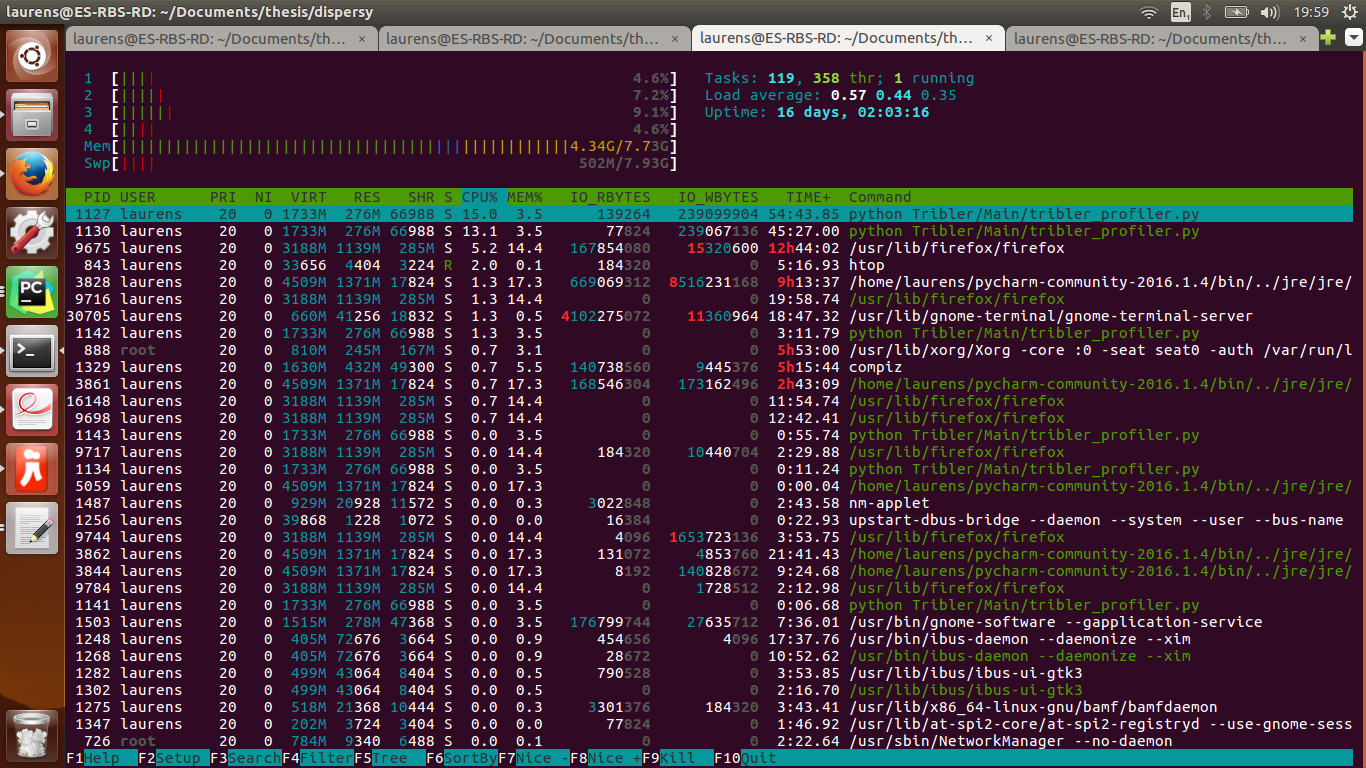
\includegraphics[width=0.95\paperwidth]{experimentation/images/htop.png}}
	\caption{The output of a four hour idle run.}
	\label{fig:htop_io_idle_run}
\end{figure} 

The results are visible in Figure~\ref{fig:htop_io_idle_run}. \todo{cut unity desktop}
From these results we observe that Tribler current has an IO of 144 MB/Hour.
To observe the individual components separately, we have created a breakdown the database queries performed by Tribler.
This breakdown is visible in Table Z.
As we can see, B is doing the most IO... \todo{Implement breakdown functionality and measure this.}

\section{Performance regression using Gumby}

\begin{figure}[h]
	\makebox[\textwidth][c]{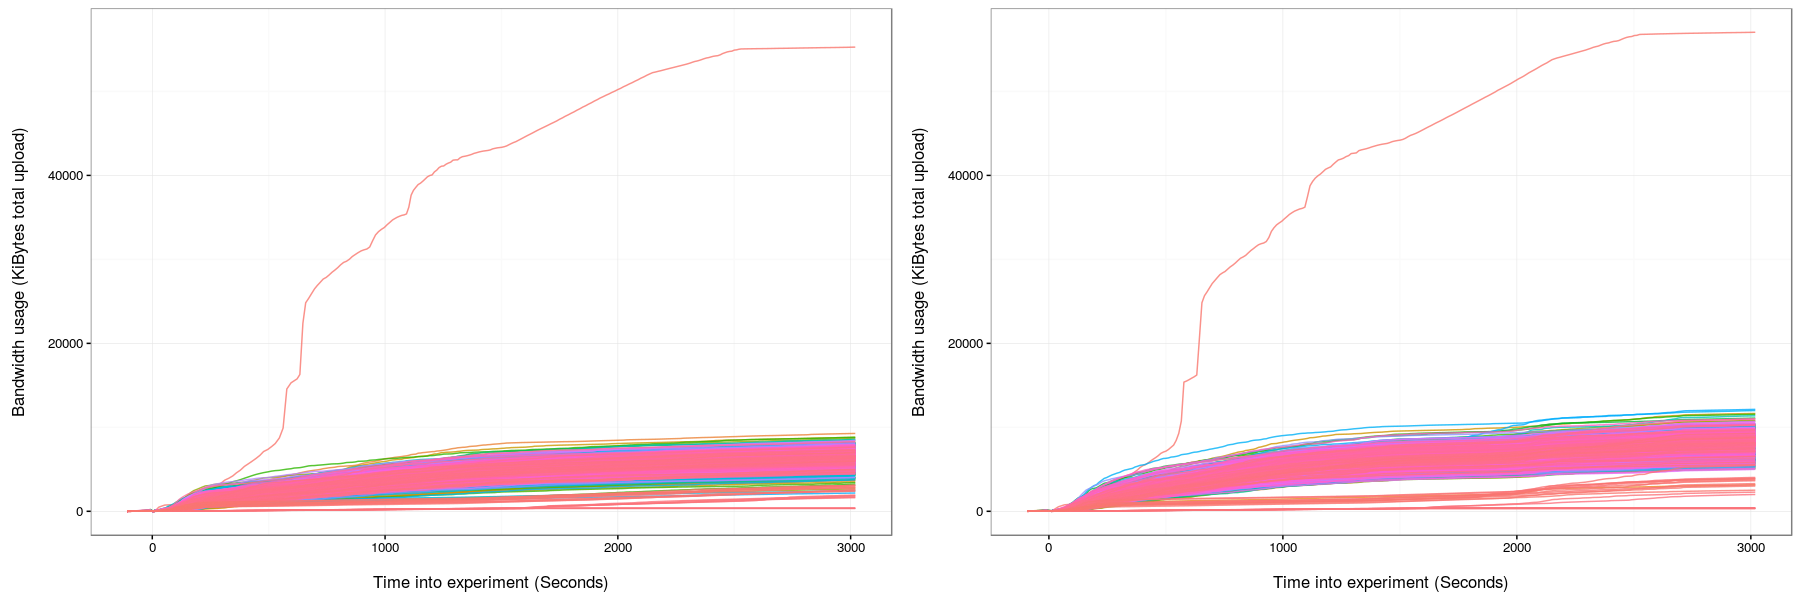
\includegraphics[width=\linewidth]{experimentation/images/send.png}}
	\caption{A side by side comparison of two \enquote{allchannel} experiment runs. Left the current code base, right asynchronous Dispersy with blocking I/O.}
	\label{fig:side_by_side_send}
\end{figure} 

Tribler has an experiment runner framework for Dispersy and Tribler: Gumby.
Using Gumby, one can specify configurations and scenario files to be executed.

Configuration files specify all the settings needed in order to run an experiment using Gumby.
The scenario file allows for a carefully timed execution of functions.
Each line in a scenario file specifies which node executes which function at what time. \todo{Example of such a scenario file? yes/no?}
Currently, Gumby is being used to run an experiment on the DAS5 super computer\footnote{\url{http://www.cs.vu.nl/das5/}}.
Whenever a push happens on a pull request on GitHub, our Jenkins continuous integration system automatically schedules this experiment to be run.

Using Gumby, statistics such as CPU, memory consumption and I/O are automatically tracked.
Any additional information that one wishes to track can be logged and parsed using auxiliary post experiment scripts.
Currently, graphs are being generated in the R programming language using the ggplot2 library.

To obtain a regression testing system, we decided to extend Gumby.
To obtain the data for comparison, the proposed commits first have to be run inside an experiment using a predetermined scenario and configuration file.
Once this experiment is done, Jenkins can fetch the data of the last successful experiment run of the current code base.
Next, using the data from both experiments we generate graphs.
By creating a side-by-side plot of two graphs using the same scales, developers can immediately see any changes, see Figure~\ref{fig:side_by_side_send}.\todo{Replace the right one with the dispersy async + non-block, should be more of a change.}

\section{Validating the performance regression system}

To validate the performance regression system, we have resolved one of Tribler's biggest bottlenecks: Dispersy's database I/O.
Dispersy performs a lot of I/O.
Currently, this I/O is blocking the main thread when waiting for the database, wasting valuable CPU cycles.
To address this problem, we have written Dispersy's I/O to become asynchronous and non-blocking.
To realize this, a new database manager \enquote{StormDBManager} is introduced and 90\%\todo{made up number, need to calculate the actual value.} of Dispersy's functions have been refactored.

\subsection{A new database manager}

\begin{figure}[h]
	\makebox[\textwidth][c]{\includegraphics[width=\linewidth]{experimentation/diagrams/storm_db_worker.png}}
	\caption{An overview of the queueing mechanism of StormDBManager.}
	\label{fig:storm_db_worker}
\end{figure}

StormDBManager features a complete asynchronous and non-blocking interface to handle database access.
It is developed using the Storm database framework which is developed by Canonical and featured in several other products such as Launchpad \cite{canonical2011storm}.
Storm allows for both an old-fashioned database approach using direct SQL statements or to use it as an object-relational mapper (ORM).
Currently, Storm supports three databases: SQLite, MySQL and PostgreSQL.
As Dispersy makes use of a SQLite3 database, this was a necessity.
Additionally, the Storm database framework has integrated support for Twisted and is available on the official repositories of Ubuntu and Debian, making it a good fit for Tribler.
Because Storm also features ORM support, this database manager can be the foundation for an ORM based approach.

Since multi-threaded support is severely limited using SQLite3, we decided to leverage the Twisted thread-pool to allocate a thread for a longer period of time to run a worker on.
This worked will be owned by the StormDBManager.
Using this approach, all database operations happen on the same thread but outside the Twisted main thread, guaranteeing I/O does not block it.
The system works as follows, visualized in Figure~\ref{fig:storm_db_worker}.
Fist, a Dispersy function calls the StormDBManager (1).
The StormDBManager generates a deferred and returns this to the caller (2).
Next, the StormDBManager queues a tuple of four elements (3):

\begin{enumerate}
	\item The function to be called, e.g. execute or fetchone.
	\item The arguments to be passed to the function.
	\item The keyword arguments to be passed to the function.
	\item A deferred to handle the response in an asynchronous way.
\end{enumerate}

Note that by using a thread-safe queue, all calls are scheduled in the same order as required, ensuring serialized behaviour.
The worker running on the thread waits blocking for new items to come, preventing the thread from dying.
Once it a tuple is available it fetches it (4).
It then executes the function (5) and calls the deferred's callback with the result (6).
After that, the worker proceeds to wait blocking for a new item, or executes the next tuple if present.
To make sure the worker can still commit or release the thread, two predetermined values can be queued upon which the worker will commit or shut down, respectively.

\subsection{Refactoring Dispersy}

As the new StormDBManager will start retuning deferreds, functions of Dispersy need to be able to coop with this new paradigm.
Every caller of this function will need to be recursively updated as well to handle the deferreds being returned.
By making extensive use of the \enquote{inlineCallbacks}\footnote{\url{http://twistedmatrix.com/documents/current/api/twisted.internet.defer.inlineCallbacks.html}} decorator, approximately 90\% of all Dispersy functions were modified. \todo{Replace 90\% with actual number.}
\todo{continue story.}
